\section{Laboratorial Testing} \label{sec:Lab}

In the laboratory, it was possible to simulate with real components the circuit in Figure \ref{fig:rc}. However, there were used some components that were not allowed for the theoretical and simulation analysis such as resistors with 2k$\Omega$ and more that three resistors of 1k$\Omega$. So the values used in the presential lab for the components were:
\begin{table}[!htb]
\centering
  \begin{tabular}{|c | c|}
    \hline    
\bf Component  & \bf Value\\ \hline 
R1  & 0.67 k$\Omega$ \\ \hline 
R2  & 1.00 k$\Omega$ \\ \hline 
R3  & 100.00 k$\Omega$ \\ \hline 
R4  & 0.50 k$\Omega$ \\ \hline 
C1  & 220.00 nF \\ \hline 
C2  & 220.00 nF \\ \hline 

\end{tabular}
 \caption{Components used in the laboratory}\label{tab:labb}
\end{table}

With $R_2$= 1k $\Omega \parallel$ 1k$\Omega$ and $R_4$= 1k$\Omega \parallel 2k\Omega$.

The results obtained were, for a frequency of f = 1 kHz: 

\begin{align*}
  v_i &= 64.0\ mV \\
  v_o &= 5.9\ V \\
  Gain &\approx 92.2 \\
  Gain_{dB} &\approx 39.3 dB\\
\end{align*}

These values aren't exactly the expected due to the manufacturer's tolerance of the capacitors and resistors used.


Altough we didn't use this exact values for the components used, the laboratory work helped to understand how the circuit works and the changes we will need to do, in the following analysis, to achieve the desired values.

\begin{figure}[h] \centering
  \begin{minipage}{.5\textwidth}
    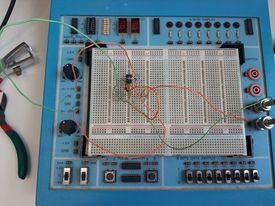
\includegraphics[width=.9\textwidth]{lab1.jpg}
    \caption{Image of the circuit built in the laboratory}
    \label{fig:simenv}
    \end{minipage}%
  \begin{minipage}{.5\textwidth}
  \centering
    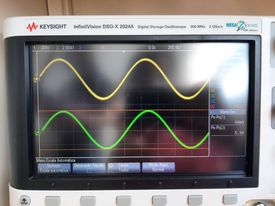
\includegraphics[width=.9\textwidth]{lab2.jpg}
    \caption{Results obtained in the osciloscope}
    \label{fig:compenv}
      \end{minipage}%
\end{figure}

\section{Theoretical Analysis} \label{sec:analysis}

\subsection{Gain and Central Frequency}
 
The transfer function that caracterizes the studied circuit is given by

\begin{equation} \label{eq:transfer}
 \text{T(s)}=\frac{\text{R\textsubscript1}}{\text{Z\textsubscript{C1}+R\textsubscript1}} \left( 1+\frac{\text{R\textsubscript3}}{\text{R\textsubscript4}}\right) \frac{\text{Z\textsubscript{C2}}}{\text{Z\textsubscript{C2}+R\textsubscript2}}
\end{equation}

where Z\textsubscript{C1} and Z\textsubscript{C2} are the capacitor's impedances.

Analysing the present circuit, it's easy to understand that the term $ 1+\frac{\text{R\textsubscript3}}{\text{R\textsubscript4}}$ is proportional to the linear voltage gain, whereas R1 and C1 control the low cut-off frequency (f\textsubscript{L}) and R2 and C2 control the high cut-off frequency (f\textsubscript{H}).

The lower and upper cut-off frequencies correspond to the frequencies 3db bellow the maximum dB gain (\input{../mat/max.tex} dB). Then, the central frequency was computed by the geometric mean:

\begin{equation}
 \text{f\textsubscript{c}}= \sqrt{\text{f\textsubscript{L}} \times \text{f\textsubscript{H}}}
\end{equation}

The results are the following:

\begin{table}[!htb]
\centering
  \begin{tabular}{|c | c|}
    \hline    
    \input{../mat/frequencies.tex}
 \end{tabular}
 \caption{Frequency Analysis}\label{tab:theo:frequencies}
\end{table}


\begin{table}[!htb]
\centering
  \begin{tabular}{|c | c|}
    \hline    
    \input{../mat/gain.tex}
 \end{tabular}
 \caption{Gain Analysis}\label{tab:theo:gain}
\end{table}

The following graphics are obtained directly from the transfer function's (\ref{eq:transfer}) magnitude and argument, respectively:


\begin{figure}[h] \centering
  \begin{minipage}{.45\textwidth}
    \includegraphics[width=.8\textwidth]{T.eps}
    \caption{Frequency response - Gain(dB)}\label{fig:theo:gain}
  \end{minipage}%
    \hspace{2 mm}
  \begin{minipage}{.45\textwidth}
  \centering
    \includegraphics[width=.8\textwidth]{Tphase.eps}
    \caption{Frequecy response - Phase (degrees)}\label{fig:theo:phase}
      \end{minipage}
\end{figure}

As we can see, there's a small offset at the central frequency,
\newpage
\subsection{Input and Output Impedances}

To compute the input and output impedances, we followed the ideal OP-AMP model : Z\textsubscript{in}=$\infty$ and Z\textsubscript{out}=0, and knowing that $\text v_- = \text v_+$ in any feedback configuration, so we achieve that:

\begin{enumerate}
 \item From the input, the capacitor C1 and the resistor R1 are being seen in series
 \item From the output, the capacitor C2 and the resistor R2 are being seen in parallel
\end{enumerate}

arriving at the following equations:


\begin{equation}\label{impedances}
\begin{cases}
    \text{Z\textsubscript{in}} = \frac{\text v_\text I}{\text i_\text I}\Bigr|_{\text{Z\textsubscript L}=\infty} = \text{Z\textsubscript{C1}+R\textsubscript{1}}\\
    
    \\
    
    \text{Z\textsubscript{out}} = \frac{\text v_\text o}{\text i_\text o}\Bigr|_{\text v_\text I=0} =  \text{Z\textsubscript{C2}} \parallel \text{R\textsubscript{2}}  \\

 \end{cases}
\end{equation}


%  Considering that:
%  
%  \begin{equation}
%  \begin{cases}
%     v_- = v_+ = \frac{R1}{R1+Z_{C1}} v_i\\
%     v_A = \left(1 + \frac{R3}{R4}\right) v_-\\
%     v_o = \frac{Z_{C2}}{Z_{C2}+R2} v_A\\
%   \end{cases}
%  \end{equation}
 
 
The results are the following:

\begin{table}[!htb]
\centering
  \begin{tabular}{|c|c|}
    \hline    
    \input{../mat/impedances.tex}
 \end{tabular}
 \caption{Input and output impedances}\label{tab:theo:impedances}
\end{table}

The output impedance is smaller than the input impedance as intended.

\subsection{Overall Theoretical Results}

In the following table, there are the final result for the value of the merit, such as other results of interst:


\begin{table}[!htb]
\centering
  \begin{tabular}{|c | c|}
    \hline    
    \input{../mat/final.tex}
    \input{../mat/cost.tex}
 \end{tabular}
 \caption{Final Results Theoretical Analysis}\label{tab:theo:final}
\end{table}



